%% LaTeX source of Chapter 4 of the thesis.
%% NEVER compile this file. Complie 'thesis.tex' instead.

\chapter{时序数据压缩算法和可视化}
\label{Chapter 3}

\section{时序数据压缩算法与实现}
\label{section 3.1}
\subsection{问题描述}
\label{section 3.11}
汽车运行过程中引擎的相关参数我们可以通过传感器获得,例如汽车发动机的转速,汽车的进气量和喷油量。这些数据的维度可以达到两个数量级以上,也就是说我们采集到
的数据在数据库当中可以单个表达到100列。假设我们的采样频率为100,可以计算每小时我们采集数据的次数为3600*100.很明显如果汽车长时间运转,这些数据将
对汽车的存储系统造成极大的压力。这些数据全部存储起来将浪费大量的存储资源,但是如何不加处理的直接丢弃,那么一旦出现汽车故障,我们将不能获取即时有
效的原始数据。

通过我们对时序数据的观测,在这些时序数据中存在大量的数据冗余,原因很直接,因为大部分的数据通常在某段时间都是稳定的,例如引擎稳定运行时的温度,特别
是像汽车的档位这类数据,很有可能长时间不改变,对于日常的业务场景来说,维护人员很难从海量的时序数据中快速找到自己需要的异常数据,因此我们可以允许再
保存的过程中与原始数据有一定的误差,在存储的过程中我们依然采用了关系数据库,这不仅是因为关系数据库的技术成熟,而且目前存在的一些早期的时序数据库的实现原型也是基于关系数据库而来。


时间本身充满了多变性,他可以是一个时间点,也可以是一个时间间隔,既可以是线性的,也可以是周期的。如果考虑时序数据的维数,可想而知这样的数据他的复
杂度是相当高的,对于这样的数据,如何可视化也呈现出了多样性,根据特定的时序数据,现在已经存在了一些可视化框架,例如针对模拟数据我们可以采用SimVis,
而针对新闻数据我们可以采用ThemeRiver进行分析。

时序数据可视化从通用的角度来看可以认为是从维度到空间的映射,一般可视化框架有XmdvTool和Visage相对标准的可视化技术,而且平行坐标,复杂坐标都可以用来可视化时序数据,但对于海量的时序数据,这些框架显得捉襟见肘。

对于数据量庞大的时序数据,我们可以选择基于蜡烛图的可视化方法,蜡烛图(candlestick chart)又称k线图,K线图可以容易的表示统计数据中的若干内容,
关于K线图的具体内容请参考背景知识。


\subsection{算法的基本思路}
\label{section 3.12}

我们根据时序数据的维数和设定的压缩比例,对输入的时序数据进行单维处理。在单维数据中我们将无明显波动的数据,合并到相同的区间中,注意在合并的过程中,
同时更新对应区间的时间点,当我们每个区间的数据点数超过了限制之后,我们采用对应的区间合并算法,将每维数据进行区间合并。处理完单维数据之后,我们将
所有维数的数据进行区间合并,来产生对应的最终输出。

如图所示\ref{Figure 3-1-1}:

\begin{figure}[h!]
	\centering
	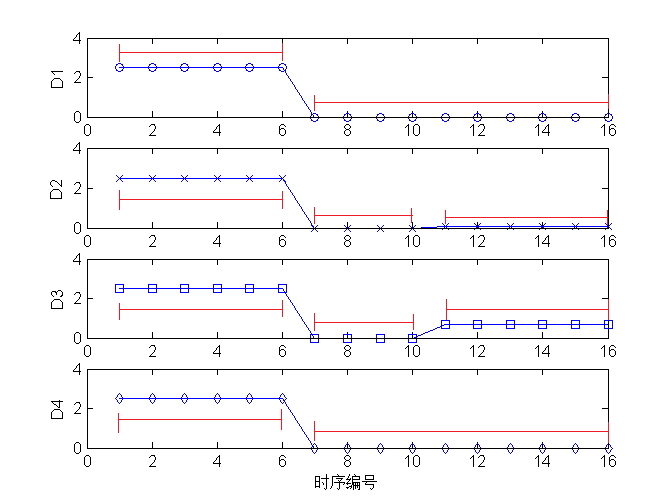
\includegraphics[scale=0.5]{./images/figure-3-1}
	\caption{时序输入数据}
	\label{Figure 3-1-1}
\end{figure}


假设我们采样到的时序数据包含4维,D1~D4,其中我们可以看到D1从t1到t6的值未发生变化,t7到t16区间内的值相同,因此我们将D1划分为[1,6]
[7,16]两个区间,对于D2~D4我们也采用相同的方法,D2和D3将被划分为3个区间[1,6]、[7,10]、[11,16].同时我们将这几个区间的时间标签提取出来并进行排序
重排后的时序列表对应为[1,6,7,10,11,16]
,然后我们重新生成时序数据,此时共产生了6个时刻对应的6条数据,每个时刻对应的值为该区间的平均值,最后通过压缩后的结果如下表所示。

\begin{center}
  \begin{tabular}{ | p{3cm} | p{3cm} | p{3cm} | p{3cm} | p{3cm} | }
    \hline
    T  & D$_{1}$ & D$_{2}$ & D$_{3}$ & D$_{4}$ \\ \hline
    1  & 2.5     & 2.5     & 2.5     & 2.5     \\ \hline
    6  &2.5      &2.5      &2.5      &2.5      \\  \hline
    7  &0.0      &0.0      &0.0      &0.0       \\ \hline
    10 &0.0      &0.0      &0.0      &0.0       \\ \hline
    11 &0,0      &0.1      &0.7      &0.0       \\  \hline
    16 &0.0      &0.1      &0.7      &0.0       \\   
    \hline
  \end{tabular}
\end{center}

\subsection{数据区间的定义}
\label{sectoin 3.13}

设D维时序数据的每一分量为D$_{i}$,压缩后的数据点数我们设置为CP(D$_{i}$),并将压缩梯度Grad(D$_{i}$)设置为CP(D$_{i}$)*2$^{k}$(k=1,2,3...)
,定义Max(D$_{i}$)为D$_{i}$已经扫描数据的最小值,Min(D$_{i}$)为D$_{i}$已经扫描过得数据最大值,IL(D$_{i}$)
用于存储已经扫描过的区间列表,列表的每一个区间是一个六元向量:


\begin{equation}
T=<t_{s},t_{e},v_{max},v_{min},v_{avg},n>
\end{equation}


其中t$_{s}$和t$_{e}$分别表示区间的开始时间标签和结束时间标签,v$_{max}$,v$_{min}$,v$_{avg}$分别表示区间类采样值的最大值,最小值,和平均值。
其中n表示所有的数据点数。每个区间是1个以上的原始数据点合并之后的结果,同一个区间覆盖的原始数据点基本平稳,而相邻的区间分隔的时间节点应该对应原始数
据中比较明显的拐点,在压缩的过程中我们在指定的输入条件CP(D$_{i}$)下,不断对D$_{i}$创建区间,扩展区间和合并区间。


\textbf{新建区间CI:}高维度的时序数据再压缩的过程中必须保持原数据总体变化趋势这些基本特征,在数据处理的过程中,当遇到较大的数据奇点且不在约定的梯度等级时,此时我们需要闯将新的区间段,新的区间段取决于奇点数据,也就是:
\begin{equation}
I_{n}=<t,t,d_{it},d_{it},d_{it},1>
\end{equation}
其中d$_{it}$为拐点数据,也就是当前时刻t的第i维的数据值。

\textbf{扩展区间EI:}在扫描数据序列的过程中,若当前数据点d$_{it}$属于当前的数据区间,则应对当前区间进行更新,区间扩展方法为:
\begin{equation}
I_{last}=<t_{s},t,MAX(v_{max},d_{it}),MIN(v_{min},d_{it}),(v_{avg}*n+d_{it})/(n+1),n+1)>
\end{equation}
其中I$_{last}$为IL(D$_{i}$)区间的最后一个元组,d$_{it}$为当前时刻t关于D$_{i}$的分量


\textbf{区间合并MI:}区间合并发生在已有的区间总数超出了设定的数据点数CP(D$_{i}$)时进行,区间合并是指将原来相邻的区间合并为一个区间,设:
\begin{equation}
I_{i}=<t_{s},t_{e},v_{max},v_{min},v_{avg},n>
\end{equation}


\begin{equation}
I_{i+1}=<t_{s}^{'},t_{e}^{'},v_{max}^{'},v_{min}^{'},v_{avg}^{'},n^{'}>
\end{equation}

为数据区间列表中相邻的元组,则合并后数据区间I$_{lr}$:

\begin{equation}
\begin{split}
I_{lf}=<MIN(t_{s},t_{s}^{'}),MAX(t_{e},t_{e}^{'}),MAX(v_{max},v_{max}^{'}),MIN(v_{min},v_{min}^{'})\\
,(v_{avg}*n+v_{avg}^{'}*n^{'})/(n+n^{'}),n+n^{'}>
\end{split}
\end{equation}


\subsection{数据压缩算法}
\label{3.14}
在对整个数据序列进行压缩的过程中,顺序扫描对应的数据,分别对每一分量进行区间压缩算法,得到所有不同分量的区间列表序列IL。在区间的创建和扩展的过程
中,对每个分量D$_{i}$判断IL(D$_{i}$)中的区间个数,和CP(D$_{i}$)的大小,如果|IL(D$_{i}$)|>CP(D$_{i}$)
则按照区间合并操作MI选择性的对相邻区间进行合并,这里的选择性是指选哪些数据,分布较为接近和相似的区间进行合并,最后,取IL中所有的IL(D$_{i}$)
中的元组标签并按时间先后进行排序,将排序好的时间标签,放入标签队列中TL,最终生成分量数据,对应的如下算法:
\newpage


\begin{algorithm}
% enter the algorithm environment
\caption{高维时序数据压缩算法CompressInterval}
% give the algorithm a caption
\label{alg1}
% and a label for \ref{} commands later
\begin{algorithmic}[1]
% enter the algorithmic environment
\REQUIRE 分量压缩点数CP(D$_{i}$),原始数据序列D 
\ENSURE 压缩后的数据序列
\FOR{($i=1$ to N)}
\STATE Max(D$_{i}$)=0;Min(D$_{i}$)=0;IL(D$_{i}$)=[];
\STATE Grad(D$_{i}$)=CP(D$_{}i$)*k;
\ENDFOR
\WHILE{(未达到输入数据D结束位置,且下一条数据记录为D$_{t}$)}
\STATE 	{\FOR{$i=1$ to $N$}
		\STATE Max(D$_{i}$)=MAX(Max(D$_{i}$),d$_{it}$);
		\STATE Min(D$_{i}$)=MIN(Min(D$_{i}$),d$_{it}$);
		\STATE I$_{last}$=IL(D$_{i}$)的最后一个区间;
		\IF{($ d_{it} \geq I_{last} \times v_{min}  \AND d_{it} \leq I_{last} \times v_{max} )$}
		\STATE $ I_{last} = EI(I_{last},d_{it}) $
		\ELSE  
		\STATE $ IL(D_{i}) push EC(d_{it}) $
		\ENDIF
		\IF{($   |IL(D_{i})|  > CP(D{i})   $)}
		\STATE $ IL(D_{i})=MergeInternal(IL(D_{i}),CP(D_{i}),Grad(D_{i})) $
		\ENDIF
		\ENDFOR
		}
\ENDWHILE
\STATE IL=[$ IL(D_{1}),IL(D_{2}...IL(D_{n}) $];
\RETURN GenData(IL);
\end{algorithmic}
\end{algorithm}


\subsection{区间合并算法}
\label{section 3.15}
时序数据压缩算法CompresInterval先对每一分量的相关数据进行初始化,在我们依次读入每条数据之后,对于每条数据我们都逐渐更新最大值最小值,根据读入值
的大小我们判断是否需要开辟一个新的区间,如果不需要开辟新的区间我们将直接对最后一个区间进行扩展,当处理完每条输入的数据之后,此时根据我们事先设定的
CP(D$_{i}$)来判断区间内部数据的值是否达到了极限,当区间内部的数据点超过我们设定的值后,我们就可以使用区间合并算法来生成新的数据。对应的区间合并算法如下所示:

\begin{algorithm}
% enter the algorithm environment
\caption{区间合并算法IntervalMerge}
% give the algorithm a caption
\label{alg2}
% and a label for \ref{} commands later
\begin{algorithmic}[1]
% enter the algorithmic environment
\REQUIRE 需要合并前的区间列表IL(D$_{i}$),CP(D$_{i}$),Grad(D$_{i}$) 
\ENSURE 通过合并算法之后产生的新的区间列表IL(D$_{i}$)
\STATE  R(D$_{i}$)=(Max(D$_{i}$)-Min(D$_{i}$))/Grad(D$_{i}$)
\FOR{($i=1$ to |IL(D$_{i}$)-1|)}
\STATE{	\IF {$( \exists x <Grad(D_{i}) \AND I_{i}.v_{min} \geq  Min(D_{i})+x*R(D_{i}) \AND I_{i}.v_{max}<Min(D_{i})+(x+1)*R(
		D_{j}) \AND I_{i+1}.v_{min} \geq Min(D_{i})+x*R(D_{i}) \AND I_{i+1}.v_{max}<Min(D_{i})+(x+1)*R(D_{i}))$}
		\STATE $I_{i}=MI(I_{i},I_{i+1})$
		\ENDIF
	}
\ENDFOR

\WHILE {$(|IL(D_{i})|>CP(D_{i}))$}
\STATE{	\STATE $Grad(D_{i})=Grad(D_{i}/2)$
		\STATE $ R(D_{i})=(Max(D_{i})-Min(D_{i}))/Grad(D_{i})$
		\FOR   {$i=1 to |IL(D_{i})|$}
		\STATE{
			\IF{$( 	 \exists x <Grad(D_{i}) \AND I_{i}.v_{min} \geq  Min(D_{i})+x*R(D_{i}) \AND I_{i}.v_{max}<Min(D_{i})+(x+1
			)*R(D_{j}) \AND I_{i+1}.v_{min} \geq Min(D_{i})+x*R(D_{i}) \AND I_{i+1}.v_{max}<Min(D_{i})+(x+1)*R(D_{i})    )$}
			\STATE $I_{i}=MI(I_{i},I_{i+1})$
			\ENDIF
		}
		\ENDFOR
}
\ENDWHILE
\RETURN IL(D$_{i}$)
\end{algorithmic}
\end{algorithm}


\subsection{数据生成算法}
\label{section 3.16}

根据事先设置的梯度Grad(D_${i}$),来判断数据点D$_{i}$,能否插入到设定的区间,当合并完成之后,如果计算出IL(D$_{i}$)仍然是大于CP(D$_{i}$),则
通过降低Grad的值来重新进行合并,通过循环检测条件来判断区间是否满足最终的要求。


\begin{algorithm}
% enter the algorithm environment
\caption{数据生成算法GenData}
% give the algorithm a caption
\label{alg3}
% and a label for \ref{} commands later
\begin{algorithmic}[1]
\REQUIRE 通过区间合并算法生成的序列IL
\ENSURE 压缩后的最终数据
\STATE IL=[]
\FOR{$(i=1 to N)$}
\STATE{
	\FOR{$(j=1 to |IL(D_{i})|)$}
	\STATE $TL.push({IL(D_{i}}_{j},t_{s}))$
	\STATE $TL.push({IL(D_{i}}_{j},t_{e}))$
	\ENDFOR
	
}
\ENDFOR

\STATE 对TL中的时间标签从小到大按时间排序
\STATE 删除TL中是多余时间标签

\FOR {$(j=1 to |TL|)$}
	\STATE 对应输出TL$_{i}$所属的IL(D$_{i}$)区间的平均值
\ENDFOR
\RETURN VOID
\end{algorithmic}
\end{algorithm}

数据生成算法,首先将所有分量的时间标签放入到一个列表中,经过排序去重之后,通过遍历IL来生成新的数据,生成的新的数据结果采用的是计算出的平均值。


\section{时序数据可视化}
\label{section 3.2}

时序数据的预处理是指将时序数据转化为数据区间列表的过程,论文中定义的区间R=$<v_{s},v_{e},v_{max},v_{min},v_{avg},v_{var}>$,其中v$_{s}$
表示时序数据的开始值,v$_{e}$表示时序数据的结束值,v$_{max}$表示时序数据的最大值,v$_{min}$表示时序数据的最小值,v$_{avg}$
表示时序数据计算出的平均值,v$_{var}$表示时序数据的标准差。


对于给定的区间大小H,时序数据预处理的过程是对连续的H个数据点按照顺序进行扫描,在扫描的过程中,计算这些数据的统计信息,我们将连续的H个数据点计算出
它的最大值最小值平均值和标准差,我们选择区间的开始值,结束值,区间最大值,区间最小值,平均值和标准差作为统计信息是因为这些信息反映了一个区间内数据
的基本特征,并且这些统计数据在区间合并的操作过程中具有良好的特性,我们可以根据相邻两个区间的值,直接计算出合并之后的统计 
数据,这样就大大减少了算法的耗时。

\subsection{时序数据预处理}
\label{section 3.21}


\begin{algorithm}
% enter the algorithm environment
\caption{时序数据预处理算法PreProcess}
% give the algorithm a caption
\label{alg4}
% and a label for \ref{} commands later
\begin{algorithmic}[1]
\REQUIRE 分隔区间的大小H,原始数据序列S
\ENSURE 区间列表R
\STATE COUNTER=0
\FOR{$(d=1 to |S.length|)$}
\IF{(COUNTER\%H==0)}
\STATE 创建一个新的区间 I=<d,d,d,d,d,0>
\ELSE{
	\STATE num=(counter\%H+1)
	\STATE $I=<I.v_{s},d,MAX(I.v_{max},d),MIN(I.v_{min},d),(I.v_{avg}*num+d)/(num+1),i.var+d*d>$
	\IF{COUNTER\%H==H-1}
	\STATE $I=<I.v_{s},d,MAX(I.v_{max},d),MIN(I.v_{min},d),(I.v_{avg}*num)/(num+1),sqrt(i.var-i.v_{avg}/H)>$
	\STATE RL.push(I)
	\ENDIF
}
\STATE 
\ENDIF
\ENDFOR
\RETURN RL
\end{algorithmic}
\end{algorithm}


\subsection{时序数据可视化}
\label{section 3.22}

时序数据首先通过预处理之后,数据会被分隔为多个区间长度为H的数据区间,并存储在关系数据库当中,本论文中采取的是SQLite,之后,时序数据的可视化都可以
以这些数据为基础来完成,当然考虑到原始数据量的规模很大,因此即使压缩为指定数据区间之后,有可能区间的个数还是很多,如果我们选取区间的总数为100,并假设
所有的数据量为100万,那么压缩过后仍然有万条数据,如果全部显示肯定是不现实的,那么换一个思路,假设我们将H设置为10000,那么我们获取到的数据点数变
为了100,此时数据的局部信息丢失的情况很有可能变得严重,在算法中,我们将合并的粒度设置为灵活可变,也就是最终的区间密度可以由用户指定,

定义初始化处理完的数据为元数据,并且由于默认的区间值为H。对于每个区间我们定义 R=$<v_{s},v_{e},v_{max},v_{min},v_{avg},v_{var}>$
,设置数据的区间大小为kH,那么以kH为区间大小的区间数据我们设置为:
\begin{equation}
$R^{'}=<v_{s}^{'},v_{e}^{'},v_{max}^{'},v_{min}^{'},v_{avg}^{},v_{var}^{'}>$
\end{equation}
那么需要合并的元数据区间中,第i个数据区间的数据为:
\begin{equation}
$R=<v_{si},v_{ei},v_{maxi},v_{mini},v_{avgi},v_{vari}>$
\end{equation}
存在如下表达式:
\newline
\alpha_{s}=v_{s}
\newline
\alpha_{e}=v_{e}
\newline
\alpha_{max}=max(v_{1max},v_{2max}...v_{kmax})
\newline
\alpha_{min}=min(v_{1min},v_{2min}...v_{kmax})
\newline
\alpha = 1/k*\sum_{n=1}^Nv_{javg}
\newline
\alpha_{var}^{2}*1/k=\sum_{n=1}^kv_javg^2+\sum_{n=1}^kv_jvar^2+{\sum_{n=1}^kv_javg}^2
\newline

基于上面的公式我们可以计算出kH区间长度的数据区间特征值的方法,对于R$^{'}$中的开始值结束值最大值最小值平均值,计算都非常简洁,对于标准差的计算可
通过对应的表达式计算出,通过将$\alpha_{var}^2$与合并的k个元数据区间的方差之和做减法计算,消去原始数据即可以得到R$^{'}$的计算表达式。

